\section{Introduction}
% Large Language Models (LLMs) have demonstrated remarkable capabilities 
% in various natural language processing tasks\citep{brown2020language, chowdhery2022palm, touvron2023llama}.

% Large Language Models (LLMs) have achieved remarkable success in various 
% natural language processing tasks\citep{brown2020language, chowdhery2022palm, touvron2023llama},
% demonstrating strong reasoning abilities 
% in complex scenarios\citep{wei2022chain, kojima2023large, zelikman2022star}.
% Large Language Models (LLMs) have achieved demonstrated remarkable reasoning abilities
% in various natural language processing tasks\citep{brown2020language, }
% Despite their impressive capabilities, LLMs often struggle with hallucinations and
% factual inaccuracies\citep{ji2023survey, zhang2023survey}, particularly
% when answering questions that require specific knowledge.
% To address these challenges, 
% Knowledge Graph Question Answering (KGQA) aims to answer natural language questions
% by reasoning over large-scale knowledge graphs (KGs).

Large language models (LLMs) have demonstrated impressive capabilities
in various natural language processing tasks~\citep{Brown2020gpt3,team2023gemini,liu2024deepseek,dubey2024llama}.
Despite their success, LLMs often struggle to produce faithful reasoning in question-answering (QA) tasks~\citep{wang2023knowledge,radhakrishnan2023question}, primarily due to knowledge gaps and
their susceptibility to hallucination~\citep{ji2023survey,guan2024mitigating}. 
To this end, the reliability of LLMs in real-world QA systems remains a significant concern.

To mitigate these issues, a promising approach is to ground LLMs' responses in external and verifiable knowledge sources~\citep{lewis2020retrieval,li2023few,ren2025investigating}.
Knowledge graphs (KGs), which emerge as an ideal candidate, provide solid factual information to validate and guide the LLMs' reasoning process~\citep{luo2024rog,zhu2024llms}. 

% Knowledge Graph Question Answering (KGQA) is defined as automatically answering
% natural language questions by reasoning over the relevant relational triples in large-scale knowledge graphs.
% It is a critical task for natural language understanding, especially for
% improving the factuality and mitigating the hallucinations of large language models (LLMs)
% through grounding their reasoning on verifiable and structured facts.
% Consequently, the potential of knowledge graph question answering (KGQA) has spurred increasing research interest.
Recent KG-enhanced reasoning methods can be broadly classified into two paradigms:
rule-based methods and imitation-based methods. 
The former~\citep{sun2023thinkongraph,zhang-etal-2025-rule} typically leveraged a pre-defined set of rules to ensure the logical consistency and faithfulness during the LLM's reasoning process.
% These methods typically leverage a pre-defined set of logical rules to prune the search space at each decoding step.
The latter~\citep{zhang2022subgraph,wu2024cotkr,jiang-etal-2025-kg} mainly trained LLMs on extensive datasets to directly mimic the reasoning patterns and heuristics embedded in the demonstrations.

% The former involves directly extracting a series of relational triples which serve as candidate reasoning paths, while the latter employs an agent that constructs reasoning paths through an iterative process of querying the graphs.

% while the intention behind schema-guided KG-enhancement is to ground LLMs in factual knowledge and provide a structured reasoning framework, an over-reliance on this approach can inadvertently create a model that is more of a puppet than a partner.
% Existing methods achieved considerable success in constraining the LLM's reasoning process by known features and patterns. 
\begin{figure}[t]
    \centering
    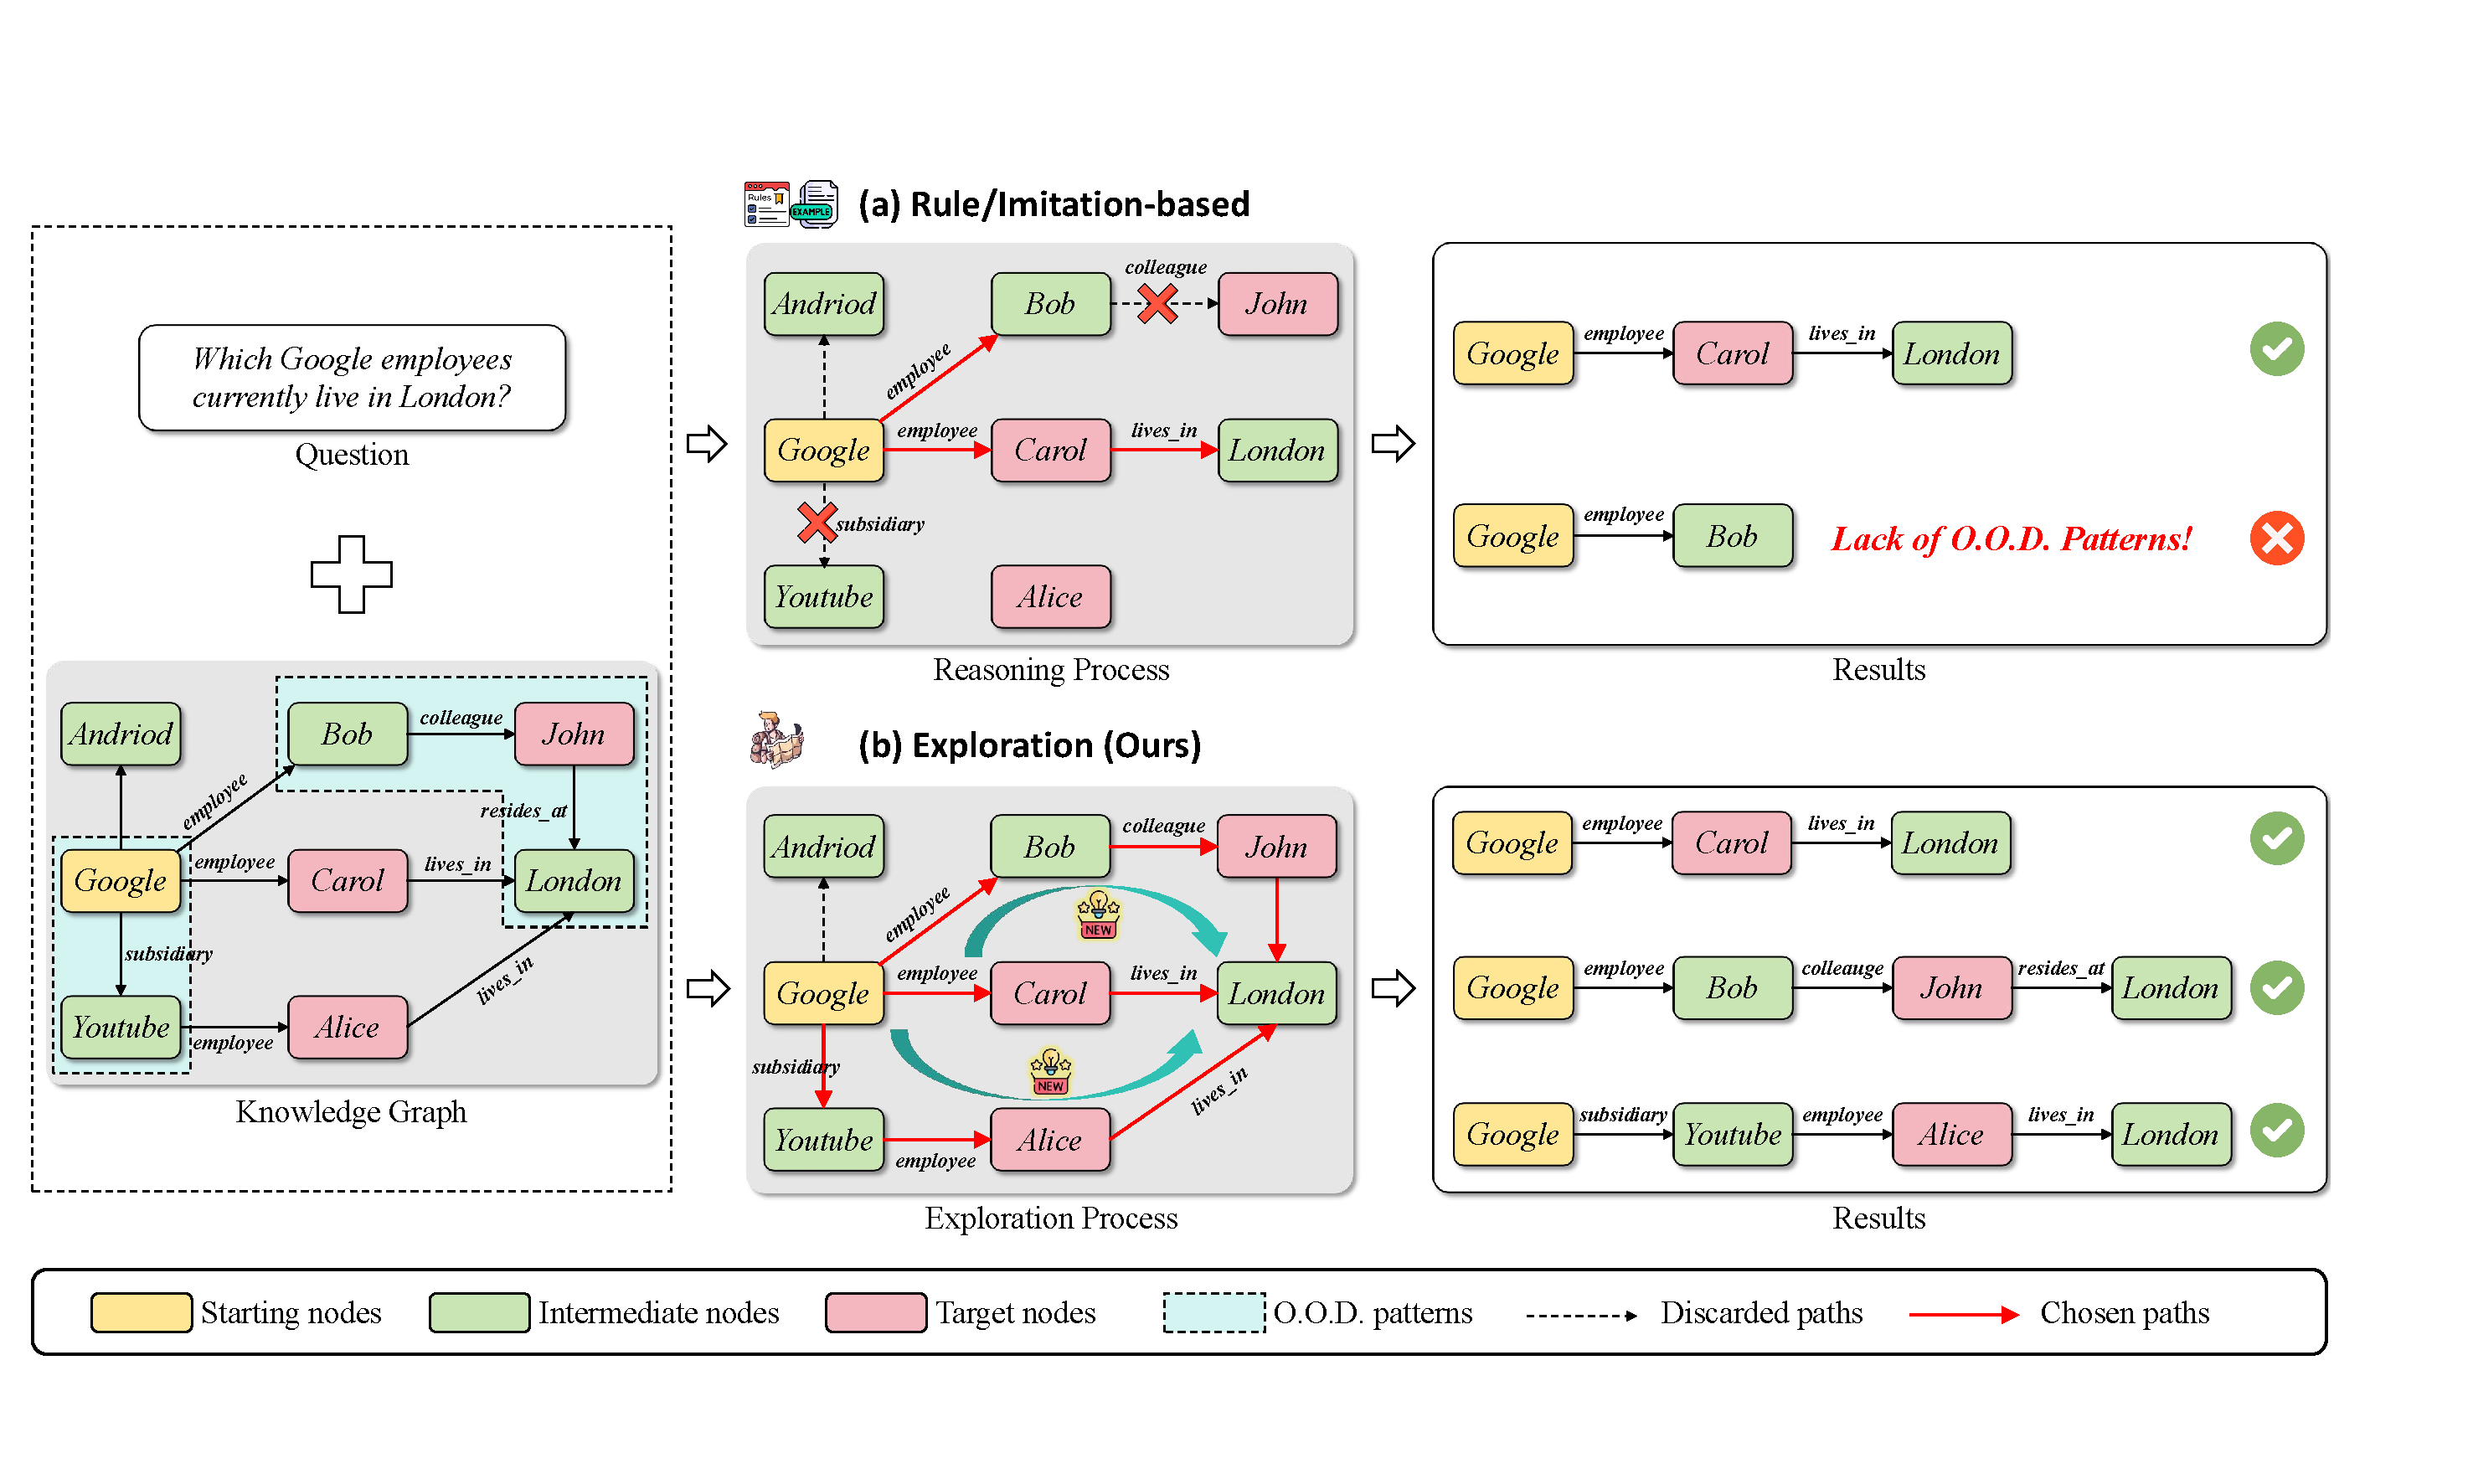
\includegraphics[width=.95\textwidth]{figures/intro0921.pdf}
    \caption{Examples of (a) rule/imitation-based method and (b) our exploration method. O.O.D. stands for Out-Of-Distribution.}
    \label{fig:intro}
\end{figure}

However, existing methods usually failed to generalize to complex graphs, especially to novel reasoning patterns that fall outside the distribution of the fine-tuning data or pre-defined rules.
For example, as shown in Figure \ref{fig:intro} (a), ``$\textit{Google}\xrightarrow{\textit{employee}}\textit{Carol}\xrightarrow{\textit{lives\_in}}\textit{London}$'' is the most common reasoning pattern corresponding to the question, and thus can be successfully recognized by existing methods. However, the patterns ``$\textit{Google}\xrightarrow{\textit{employee}}\textit{Bob}\xrightarrow{\textit{colleague}}\textit{John}\xrightarrow{\textit{resides\_at}}\textit{London}$'' and ``$\textit{Google}\xrightarrow{\textit{subsidiary}}\textit{Youtube}\xrightarrow{\textit{employee}}\textit{Alice}\xrightarrow{\textit{lives\_in}}\textit{London}$'' involve additional steps ``$\xrightarrow{\textit{colleague}}$'' and ``$\xrightarrow{\textit{subsidiary}}$'' that deviate from the most common pattern, consequently rendering them out-of-distribution and challenging for existing methods.
This observation motivates us to believe that navigating beyond the training distribution requires the capability to venture into unfamiliar regions of the graph.
For example, in Figure \ref{fig:intro}(b), although the ``$\xrightarrow{\textit{colleague}}$'' and ``$\xrightarrow{\textit{subsidiary}}$'' patterns are out of distribution, actively exploring these unfamiliar regions effectively helps discover these novel paths and give more accurate answers.
We therefore argue that a complementary capability of autonomous exploration is essential to enhance generalization in the graph reasoning task.

In this paper, we propose a novel framework named Explore-on-Graph (EoG) to incentivize autonomous exploration of LLMs on KGs.
Inspired by recent advances in large reasoning models~\citep{guo2025deepseek}, we propose to introduce reinforcement learning during training, which is preceded by a Supervised Fine-Tuning (SFT) step, to stimulate exploration capabilities.
We use the correctness of the reasoning paths' final answers as reward signals, which can be computed programmatically given the golden label.
Moreover, to improve the efficiency and semantic meaningfulness of the exploration process, we propose to incorporate path information as additional reward signals to refine the exploration strategy.
Specifically, we introduce a second dedicated training stage and leverage our proposed path-refined reward.
To evaluate the effectiveness of our approach, we conducted extensive experiments on five KGQA benchmark datasets. 
Experimental results demonstrate that our method achieves state-of-the-art performance, substantially outperforming a range of baseline methods and even surpassing the results of powerful closed-source models.
% However, existing methods usually suffered from the failure to generalize to complex graphs and unseen reasoning problems.
% This is because these approaches restrict LLMs’ reasoning process within the scope of experience and fine-tuning data, preventing it from actively exploring the vast, rich structure of knowledge graphs, which may contain novel or more efficient reasoning paths.
% For example, as shown in Figure \ref{fig:intro}(a), both rules-based and imitation-based methods neglect the unseen relation patterns ``\textit{subsidiary}'' and ``\textit{colleague}'', hence they fail to recognize the key factual reasoning paths 
% ``$\textit{Google} \xrightarrow{\textit{subsidiary}} \textit{YouTube}$'' and ``$\textit{Bob} \xrightarrow{\textit{colleague}} \textit{John}\xrightarrow{\textit{resides\_at}} \textit{London}$''.
% % Therefore, This fundamental limitation underscores the need for a new paradigm that moves beyond static rule sets and fixed demonstrations toward autonomous exploration and discovery within the knowledge graph structure.
% % This makes it difficult to 
% % thus producing factually incomplete responses. 
% Therefore, it is essential to enable LLMs to move beyond the confines of existing paradigms and achieve self-guided navigation on knowledge graphs. 

% % This static constraint prevents the model from actively exploring the vast, rich structure of the knowledge graph to find novel or more efficient reasoning paths.
% % the LLM is treated as a passive follower rather than an active explorer whether through explicit rules or implicit patterns learned from demonstrations.
% % Despite their different mechanisms, both paradigms share a common, fundamental limitation: their reliance on static, pre-defined guidance. Whether through explicit rules or implicit patterns learned from demonstrations, the LLM is treated as a passive follower rather than an active reasoner, as shown in figure x.
% % This static constraint prevents the model from actively exploring the vast, rich structure of the knowledge graph to discover novel or more efficient reasoning paths.
% % This not only leads to suboptimal performance on complex queries but also results in an inefficient utilization of the knowledge source. 
% % This fundamental limitation underscores the need for a new paradigm that moves beyond static rule sets and fixed demonstrations toward autonomous exploration and discovery within the knowledge graph structure.
% %Facilitating self-directed exploration
% To address these limitations, we propose a new exploration-based paradigm that enables LLMs to autonomously explore knowledge graphs.
% As shown in Figure \ref{fig:intro}(b), exploration-based methods can dynamically navigate through various connections and uncover multiple potential paths.
% For example, they successfully find the employees ``\textit{Alice}'' and ``\textit{John}'' by navigating through the relations ``\textit{subsidiary}'' and ``\textit{colleague}''  separately.
% The primary advantages of these methods are their capacity to gather richer contextual information and to understand complex hierarchical graph structures, 
% resulting in deeper and more comprehensive reasoning answers to the user's question.

% we advocate for a paradigm shift: from  governing the LLM's reasoning process to empowering it with the ability to autonomously explore the knowledge graph.
% In this paper, we introduce a novel framework named Explore-on-Graph (EoG), which introduces the path-refined reward modeling to incentivize autonomous exploration of LLMs over knowledge graphs.
% To effectively steer the exploration process of large language models (LLMs) toward factually grounded reasoning paths, EoG incorporates a dual-reward mechanism consisting of an answer-oriented reward and a path-refinement reward. 
% The answer-oriented reward encourages the model to generate diverse reasoning trajectories that may lead to correct answers,
% while the path-refinement reward assesses the logical coherence of each reasoning step,
% thereby mitigating hallucinations and improving the overall robustness of the reasoning process.
% To evaluate the effectiveness of our approach, we conducted extensive experiments on five knowledge graph question answering (KGQA) benchmarks. 
% The results show that our method achieves state-of-the-art performance, surpassing even commercial large-scale models. 
% Moreover, The following advantages of EoG are examined and illustrated through a number of well-designed experiments: 
% (1) EOG achieves deep exploration on knowledge graphs by LLMs.
% (2) EOG demonstrates outstanding performance in terms of reasoning depth and comprehensiveness.
% (3) EOG exhibits robust generalization capabilities across diverse datasets.

% Our approach is built upon several key innovations. First, we model the entire graph reasoning process as the generation of a long-form chain-of-thought, which fully leverages the LLM's powerful intrinsic reasoning capabilities. Second, we develop a novel reinforcement learning algorithm, Group Relative Policy Optimization (GRPO), which incentivizes the model to learn from a diverse range of explorations rather than just a single "correct" path. Finally, we design a path-refined reward model that provides a more nuanced and accurate learning signal by assessing the quality of the entire reasoning path, not just the final answer. This comprehensive feedback loop effectively guides the LLM toward generating more logical, coherent, and effective reasoning strategies.

% Our contributions can be summarized as follows:
% \begin{itemize}
%     \item{We propose EOG, a new framework that enables LLMs to autonomously explore knowledge graphs for reasoning tasks, moving beyond the limitations of pre-defined schemas.}
%     \item{We introduce Group Relative Policy Optimization (GRPO), a tailored reinforcement learning algorithm that effectively learns from diverse exploration experiences.}
%     \item{We design a path-refined reward model that provides fine-grained supervision, significantly improving the quality of the learned reasoning paths.}
%     \item{We conduct extensive experiments on four challenging KGQA benchmark datasets, demonstrating that EOG achieves new state-of-the-art results and showcasing the potential of autonomous exploration in KG-based reasoning.}
% \end{itemize}






% However, they suffer from ignoring the global structure of the knowledge graph during its inference phase, which is caused by decoupling the generation of reasoning paths from the subsequent answer inference based on those paths.

% However, recent KG-enhanced methods primarily decouple the generation of reasoning paths from
% the subsequent answer inference based on those paths, preventing LLMs from
% comprehensively understanding the original graph structure and limiting their ca-
% pacity for active exploration of the knowledge graph.





 


